\documentclass{standalone}

\usepackage{pgfplots}

\pgfplotsset{compat=1.9}

% \usetikzlibrary{}
% \usepgfplotslibrary{}

\usepackage{pgfplotstable}
\usepackage{booktabs}
\usepackage{array}
\usepackage{colortbl}

\begin{document}

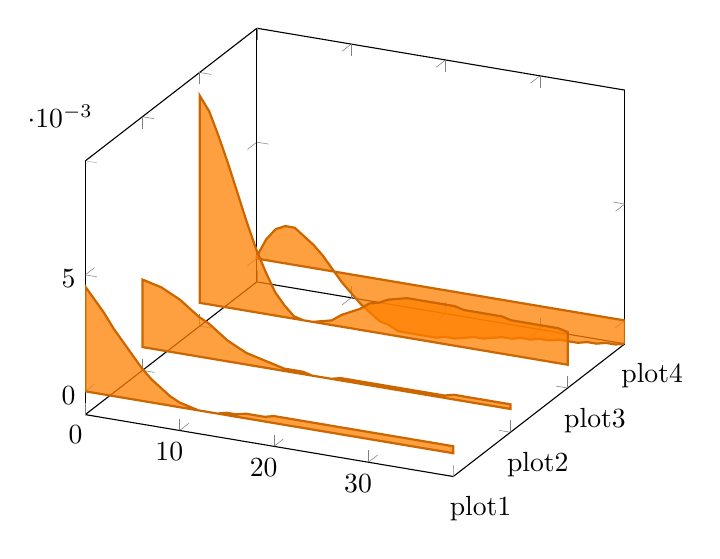
\begin{tikzpicture}

\pgfplotstableread{
plot1     plot2     plot3     plot4
0.0045    0.0029    0.0089    0.0001
0.0040    0.0028    0.0083    0.0009
0.0035    0.0027    0.0073    0.0014
0.0029    0.0025    0.0062    0.0016
0.0024    0.0023    0.0050    0.0016
0.0019    0.0020    0.0038    0.0013
0.0014    0.0017    0.0027    0.0010
0.0010    0.0015    0.0018    0.0006
0.0007    0.0012    0.0010    0.0001
0.0004    0.0009    0.0005   -0.0004
0.0002    0.0007    0.0001   -0.0008
0.0001    0.0005   -0.0000   -0.0012
0.0000    0.0004   -0.0000   -0.0015
0.0000    0.0003    0.0001   -0.0018
0.0000    0.0002    0.0002   -0.0019
0.0001    0.0001    0.0005   -0.0021
0.0001    0.0001    0.0007   -0.0021
0.0002    0.0001    0.0009   -0.0021
0.0002    0.0000    0.0012   -0.0021
0.0002    0.0000    0.0013   -0.0021
0.0003    0.0000    0.0015   -0.0020
0.0003    0.0001    0.0016   -0.0020
0.0003    0.0001    0.0017   -0.0019
0.0003    0.0001    0.0017   -0.0018
0.0003    0.0001    0.0017   -0.0018
0.0003    0.0001    0.0017   -0.0017
0.0003    0.0001    0.0017   -0.0016
0.0003    0.0001    0.0017   -0.0016
0.0003    0.0001    0.0016   -0.0015
0.0003    0.0001    0.0016   -0.0015
0.0003    0.0001    0.0016   -0.0014
0.0003    0.0001    0.0016   -0.0014
0.0003    0.0001    0.0016   -0.0013
0.0003    0.0002    0.0015   -0.0013
0.0003    0.0002    0.0015   -0.0013
0.0003    0.0002    0.0015   -0.0012
0.0003    0.0002    0.0015   -0.0012
0.0003    0.0002    0.0015   -0.0011
0.0003    0.0002    0.0015   -0.0011
0.0003    0.0002    0.0014   -0.0010
}\tabledata
\begin{axis}[
    zmin=-0.001,
    area plot/.style={
        fill opacity=0.75,
        draw=orange!80!black,thick,
        fill=orange,
        mark=none,
    },
	ytick={1,...,4},
	yticklabel=plot\pgfmathprintnumber{\tick},
]
\pgfplotsinvokeforeach{4,3,...,1}{
    \addplot3 [area plot] table [x expr=\coordindex, y expr=#1, z=plot#1]
      {\tabledata} \closedcycle;
}
\end{axis}
\end{tikzpicture}

\end{document}

